%!TEX encoding = UTF-8 Unicode
%!TEX root = shuron.tex

%% -------------------------------------------------------- %%
%%   池原研究室 2017 年度用卒業論文・修士論文テンプレート   %%
%% -------------------------------------------------------- %%
% 
%  必要なファイル
%  (基本的にファイル移動をせず,このフォルダ内のファイルを直接
%   編集することをおすすめします)
%
%  ・shuron.tex        :  このファイル,TeX ソースの本体
%  ・ikelab-thesis.sty :  卒論 / 修論スタイルにするための各種設定
%                         このファイルを編集する必要は基本的にありません
%  ・preamble.tex      :  各種パッケージのインクルードを行います
%  ・cites.bib         :  参考文献エントリファイル BibTeX で参考文献
%                         リストを出力する場合に必要です
%  ・本文中で挿入している各種画像ファイル
%    (ここでは figure ディレクトリにすべてまとめてあります)
%
\documentclass[dvipdfmx,report,disablejfam,nosetpagesize,12pt]{jsbook}

%% 卒論・修論のスタイル
\usepackage[master]{ikelab-thesis}

%!TEX encoding = UTF-8 Unicode
%
% 卒論 / 修論用 プリアンブル
%

%% フォント
\usepackage{lmodern}
\usepackage[scale=0.95]{tgheros}
\usepackage{textcomp}
\usepackage[scaled=0.85]{beramono}
\usepackage[T1]{fontenc}

%% パッケージ
\usepackage[cmex10]{amsmath}
\usepackage{amssymb,amsfonts,mathtools,bm}

\usepackage{graphicx,color}
\usepackage[table]{xcolor}

\usepackage[pdfborder={0 0 0}]{hyperref}
\usepackage{pxjahyper}

% caption のコロン「図4.4: キャプション」を「図4.4 キャプション」に直す
\usepackage[labelsep=quad,compatibility=false]{caption}
\usepackage[belowskip=1.2em]{subcaption}

\usepackage{cite,url,array,makecell}
\usepackage{algorithm,algorithmic}

% 数学コマンドの補完
\DeclareMathOperator*{\sinc}{sinc}
\DeclareMathOperator*{\prox}{prox}
\DeclareMathOperator*{\argmin}{argmin}
\DeclareMathOperator*{\argmax}{argmax}

% 参考文献表示スタイルを変更
\bibliographystyle{sieicej}

% 赤色を少し暗くする
\definecolor{red}{rgb}{0.75,0,0}

\makeatletter
   % アルゴリズム図キャプションの表記を「Algorithm」→「アルゴリズム」に
   \renewcommand{\ALG@name}{アルゴリズム}
\makeatother

% 修正箇所に色付けするコマンド
%
% ・ コマンド版
%   \fixed{修正箇所}
%
% ・ 環境版
%   \begin{fixedregion}
%      修正箇所
%   \end{fixedregion}
\newcommand{\fixed}[1]{#1} 
\newenvironment{fixedregion}{\ignorespaces}{\ignorespacesafterend}
% 下の 2 行をコメントアウトすることで色付けを無効化します
\renewcommand{\fixed}[1]{\textcolor{red}{#1}}
\renewenvironment{fixedregion}{\protect\leavevmode\color{red}\ignorespaces}{\ignorespacesafterend}

% 強調
\newcommand{\strong}[1]{\textcolor{red}{\textbf{#1}}}



%% 論文タイトル
\title{2017年度 卒論/修論テンプレート}
%% 論文英語タイトル
\etitle{The Template for Master Thesis}
%% 論文著者
\author{池研 太郎}
%% 学籍番号
\id{8XXXXXXX}
%% 指導教員名
\teacher{池原雅章\hspace{1em}教授}
%% 年月
\date{\number\year 年 3 月}
%% 所属
\department{慶應義塾大学院理工学研究科\\総合デザイン工学専攻}

% ------------------------------------------------------------------
\begin{document}

\frontmatter

% 表紙用タイトルの出力
\maketitleforcover

% タイトルを出力
\maketitle

% 論文要旨
\begin{abstract}
% 800 字程度で記述
このテンプレートは 2017 年度,池原研究室向け卒業論文・修士論文の
テンプレートです.
奥村晴彦氏による \pLaTeXe 向け jsbook ドキュメントクラスをベースに,
表紙・章のスタイル等の変更を行っています.Windows 版 \TeX\ Live 2016,
Mac OS X 向け Mac \TeX\ 2016 にて動作確認を行っています.
\end{abstract}

% 論文英語要旨
\begin{eabstract}
% 400 語程度で記述
This template is intended for the graduate/master thesis papers in 2017's 
school year, Ikehara Laboratory.
It is based on Okumura's jsbook documentclass for \pLaTeXe, and
it contains some changes on the styles for the title page and the section headers.
This template works on \pLaTeX\ engine, bundled in \TeX\ Live 2016 on Windows,
or Mac \TeX\ 2016 on Mac OS X.
\end{eabstract}

% 目次を出力
\tableofcontents

% ページ番号を数字 1 から振り直す
\mainmatter

%%%%%
% ------------------------------------------------------------------
\chapter{序論}
\section{研究目的}
このテンプレートは 2017 年度池原研究室卒業論文・修士論文用のテンプレートです.
簡単な使い方の説明を第\ref{Chap.basis}章に記しています.

\section{研究背景}
\subsection{研究背景の節}
(ここに研究背景を書く)
\subsection{研究背景の節}

% ------------------------------------------------------------------
\chapter{基礎理論} \label{Chap.basis}
\section{このテンプレートについて} \label{Sec.basis}
このテンプレートは \LaTeX の和書向けドキュメントクラス jsbook を元に,
卒業論文および修士論文向けにタイトルと章の表示スタイルに変更を
行ったものです.

\section{フォルダ構成とソースファイルについて}
このテンプレートのメインソースファイルは
``sotsuron.tex'' (卒論) または ``shuron.tex'' (修論) です.
それ以外に設置しているソースファイルや画像ファイルもこのテンプレート
において必要になるため,このファイルを移動するときは
\textcolor{red}{フォルダ構造を保ったままファイルを移動してください}.
また\textcolor{red}{ソースファイル名に日本語名を用いないでください}.
日本語ファイル名を含む \TeX ファイルは,
Windows -- Mac 間でファイルを交換した際にタイプセットできなくなる
トラブルが発生します.

\section{インクードされているパッケージについて}
preamble.tex の中でいくつかの主要なパッケージをインクルードしています.
preamble.tex 読み込みより後に同じパッケージを再度インクードしようとすると
エラーになる場合が存在するので注意してください.

\subsection*{amsmath, amssymb, amsfonts}
アメリカ数学会の開発した数式に関する拡張パッケージ,\verb+align+ 環境,
数式中の\ \verb+\text+ コマンドなどが定義されています.

\subsection*{bm}
数式中でベクトルなどに用いる太字,斜体の文字を出力する\ \verb+\bm+ 
コマンドを定義します.
\begin{equation}
   \bm{x}\ \bm{y\ z}\ \bm{A\ B\ C}\ \bm{\alpha\ \beta\ \gamma}
\end{equation}

\subsection*{color}
\textcolor{red}{色付き}の\textcolor{blue}{文字}を\textcolor[rgb]{0,0.5,0}{出力}します.

\subsection*{graphicx}
図を出力します.図の書き方は\ref{Sec.basis.fig}節を参照.

\subsection*{caption}
図表のキャプションのスタイルを制御します.

\subsection*{subcaption}
複数の図を貼り付けた時にそれぞれの図にキャプションを付ける\ \verb+\subcaption+
などのコマンドを定義します.使い方は\ref{Sec.basis.fig}節を参照.
同様の機能を持つパッケージ subfigure / subfig は非推奨です.

\subsection*{cite}
複数の参考文献を同じ箇所で引用した時に参考文献番号をソートして整理してくれる
パッケージです.
% \cite{文献1,文献2,文献3} のように複数の引用を cite コマンドの中に入れられます
(\cite{Keys1981},\cite{Hou1978},\cite{Jensen1995},\cite{Xin2000},
\cite{Muresan2004}
$\rightarrow$ \cite{Keys1981,Hou1978,Jensen1995,Xin2000,Muresan2004};
\cite{Hou1978},\cite{Carey1999},\cite{Zhang2006},\cite{Muresan2004}
$\rightarrow$ \cite{Hou1978,Carey1999,Zhang2006,Muresan2004,Yoneji2005,Takagi2016})

\subsection*{multicols}
文章の途中で 2 段組,3 段組を構成できる\ \verb+multicols+ 環境を定義します.

\section{テンプレート}

\subsection{数式}
\verb+equation+ 環境を使って次のように書きます.
\begin{equation}
   y_i = \sum_{1\leq t\leq 4} a_t x_{i\diamond t}^{(8)} + v_i
   % 後で参照するためのラベル.他の式と被らないような名前にします
   \label{eq:singleline}
\end{equation}

複数行に渡る数式は \verb+align+ 環境を使います.
\begin{align}
   \hat{\bm{y}} = \argmin_{\bm{y}}
   \left\{
      \sum_{i\in W}
         \left\|
            y_i - \sum_{i\leq t\leq 4} a_t x_{i\diamond t}^{(8)}
         \right\|
   \right.
   + &          % 揃えたい位置に & を入れる
      \sum_{i\in W}
         \left\|
            x_i - \sum_{i\leq t\leq 4} a_t y_{i\diamond t}^{(8)}
         \right\|
   \nonumber \\ % 番号なしの改行
   + &
   \lambda  
   \left.
      \sum_{i\in W}
         \left\|
            y_i - \sum_{i\leq t\leq 4} b_t y_{i\diamond t}^{(4)}
         \right\|
   \right\}
   \label{eq:multiline}
\end{align}
入門書や解説サイトにある \verb+eqnarray+ 環境は非推奨です.
数式に \verb+\label+ でラベルを貼ることで,式\eqref{eq:singleline},\eqref{eq:multiline}
のように,\verb+\eqref+ コマンドで参照することができます.

\subsection{図}
\label{Sec.basis.fig}
図は PNG, JPEG, PDF 形式がサポートされています.
BMP ファイルやその他の画像形式は,MATLAB や画像処理ソフトで PNG 形式に変換して
使用してください.


画像処理の入力・出力画像には PNG 形式を,
Inkscape や Microsoft Office で作成した図の取り込みには PDF 形式をおすすめします.
MATLAB の Figure から出した図の保存には EPS か PNG 形式がよいでしょう.
imagesc や surf で出した図を EPS 形式で保存すると非常に大きなファイルになって
しまうので適宜使い分けてください.

各形式の図のサンプルを
図\ref{Fig.example-pdf} $\sim$ 図\ref{Fig.example-3x2-grid} に示します.

\textcolor{red}{図のファイル名,格納ディレクトリ名に日本語名は用いないでください.}
また
``result.11-12.pdf'' のような
\textcolor{red}{拡張子以外の部分にドット ( . ) を含むファイル名を使用しないでください.}
Windows -- Mac 間でファイルを交換した時にタイプセットができなくなる場合があります.

\begin{figure}[tp]
   % center 環境で中央寄せする解説サイトをよく見ますが
   % 図の上下に不必要なスペースが空いてしまうので非推奨です
   % \centering を使ってください
   \centering
   % .7\hsize --> 本文の横幅の 0.7 倍
   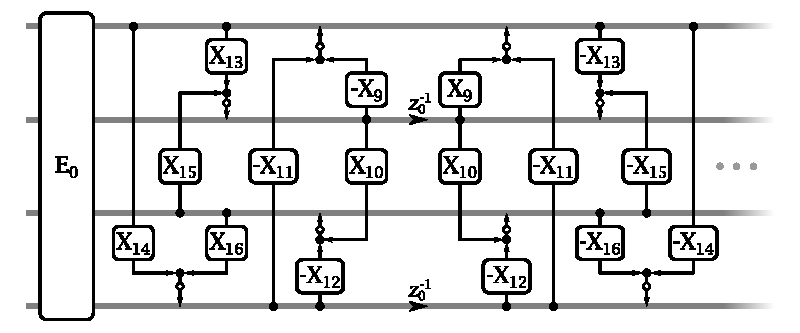
\includegraphics[width=.7\hsize]{figure/example-pdf.pdf}
   \caption{pdf 形式の図の挿入}
   \label{Fig.example-pdf}
\end{figure}

\begin{figure}[tp]
   \centering
   % ページ幅の 0.45 倍の幅をもつ minipage を横に並べて図を並置
   \begin{minipage}[c]{.45\hsize}
      \centering
      % .6\hsize --> minipage の幅の 0.6 倍
      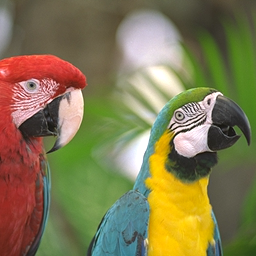
\includegraphics[width=.6\hsize]{figure/example-png.png}
      \subcaption{PNG 形式の図の挿入}
      \label{Fig.example-subcaption.a}
   \end{minipage}
   \begin{minipage}[c]{.45\hsize}
      \centering
      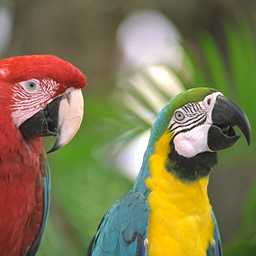
\includegraphics[width=.6\hsize]{figure/example-jpg.jpg}
      \subcaption{JPEG 形式の図の挿入}
      \label{Fig.example-subcaption.b}
   \end{minipage}
   \caption{subcaptionを用いた複数の図へのcaptionの付け方}
   \label{Fig.example-subcaption}
\end{figure}

% 3行2列に図を並べたページを作成する例
\begin{figure}[p]
   \centering
   \begin{minipage}[c]{.47\hsize}
      \centering
      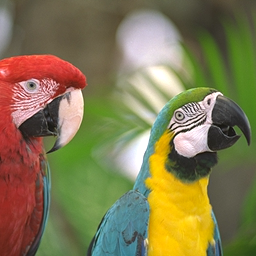
\includegraphics[width=.8\hsize]{figure/example-png.png}
      \subcaption{あ}
   \end{minipage}
   \begin{minipage}[c]{.47\hsize}
      \centering
      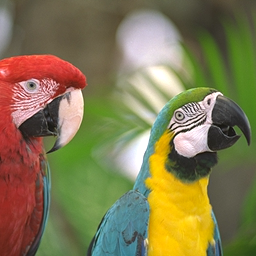
\includegraphics[width=.8\hsize]{figure/example-png.png}
      \subcaption{い}
   \end{minipage}
   \begin{minipage}[c]{.47\hsize}
      \centering
      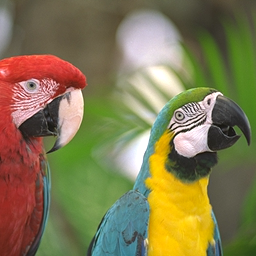
\includegraphics[width=.8\hsize]{figure/example-png.png}
      \subcaption{う}
   \end{minipage}
   \begin{minipage}[c]{.47\hsize}
      \centering
      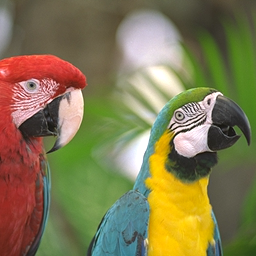
\includegraphics[width=.8\hsize]{figure/example-png.png}
      \subcaption{え}
   \end{minipage}
   \begin{minipage}[c]{.47\hsize}
      \centering
      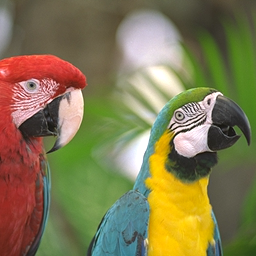
\includegraphics[width=.8\hsize]{figure/example-png.png}
      \subcaption{お}
   \end{minipage}
   \begin{minipage}[c]{.47\hsize}
      \centering
      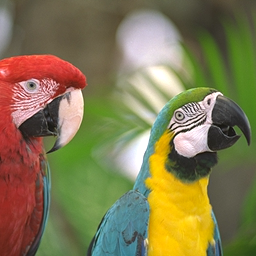
\includegraphics[width=.8\hsize]{figure/example-png.png}
      \subcaption{か}
   \end{minipage}
   \caption{3行2列に画像を配置する例}
   \label{Fig.example-3x2-grid}
\end{figure}

\subsection{表}
表組みのサンプルを表\ref{Tbl.example}に示します.
ただし印刷領域に対してサイズが大き過ぎると思うので
\ \verb+\small+ コマンドなどを用いて全体を縮小して表示すると良いかもしれません.
Excel のような,表のセル結合を \LaTeX で実現するのは非常に難しいです.
なるべくセルを結合しなくて済むように表現の工夫をした方が良いと思います.

\begin{table}[t]
   \centering
   \caption{表のサンプル}\label{Tbl.example}
   % 文字サイズを小さく
   \small
   \begin{tabular}{c|ccc}
      \hline
      \textbf{Image}  & Bicubic  & $\cdots$ & 提案手法 \\
      \hline
      \textbf{Lena}   & 33.92    & $\cdots$ & \textcolor{red}{34.74} \\
      \textbf{Flower} & 32.30    & $\cdots$ & \textcolor{red}{32.51} \\
      \textbf{Leaves} & 30.52    & $\cdots$ & \textcolor{red}{32.16} \\
      $\vdots$        & $\vdots$ & $\cdots$ &    $\vdots$        \\\hline
      平均            & 29.87    & $\cdots$ & \textcolor{red}{30.51} \\\hline
   \end{tabular}
\end{table}

\subsection{アルゴリズム図}
アルゴリズム図(擬似コード)を表記する例をアルゴリズム~\ref{Alg.example} に示します.
擬似コードはプログラムのコードを記述するためのものではありません.
自分の手法を説明するにあたって本当に擬似コードが必要かどうかよく考えて利用してください.

\begin{algorithm}[t]
   \caption{アルゴリズム図記述の例}
   \label{Alg.example}
   % algorithmic 環境の使い方は以下のページを参照してみてください
   %   http://www.biwako.shiga-u.ac.jp/sensei/kumazawa/tex/algorithmic.html
   %   http://mirrors.ctan.org/macros/latex/contrib/algorithms/algorithms.pdf (英語)
   \begin{algorithmic}[1]
      % 初期条件
      \REQUIRE{$n \geq 0 \vee x \neq 0$}
      \ENSURE{$y = x^n$}
      % 普通の文
      \STATE $y \leftarrow 1$
      % 条件分岐
      \IF{$n < 0$}
         \STATE $X \leftarrow 1 / x$
         \STATE $N \leftarrow -n$
      \ELSE
         \STATE $X \leftarrow x$
         \STATE $N \leftarrow n$
      \ENDIF
      % ループ
      \WHILE{$N \neq 0$}
         \IF{$N$ is even}
            \STATE $X \leftarrow X \times X$
            \STATE $N \leftarrow N / 2$
         \ELSE[$N$ is odd]
            \STATE $y \leftarrow y \times X$
            \STATE $N \leftarrow N - 1$
         \ENDIF
      \ENDWHILE
      % 返り値
      \RETURN{$y$}
   \end{algorithmic}
\end{algorithm}

\section{参考文献について}
参考文献リストの出力に\BibTeX を使います.
テンプレートのファイル \verb+cites.bib+ に\BibTeX のエントリーを追加してください.
日本語の文献を参考文献に加えるには\BibTeX の代わりにp\BibTeX を用いるための
設定が必要です.

% ------------------------------------------------------------------
\chapter{従来法} \label{Chap.previous}
\section{数式記述のためのTips}

\subsection{注意点}
\begin{itemize}
   \item 物理量にあたるもの(座標 $x$, $y$,時刻 $t$など)は必ず数式として記述してください.
   \item $8\times8$ の様に $\times$ を用いる表現は前後の数字も数式に入れてください.
   \item 中点の位置は,その前後の高さに合わせます %
         % , に囲まれた部分は \ldots で
         $1,2,\ldots,n$,
         % + に囲まれた部分は \cdots で
         $1+2+\cdots+n$
   \item $\sin$, $\cos$, $\exp$, $\log$, $\min$, $\max$ などのオペレーターは
         専用のコマンドを用いて立体で表記してください.
         このテンプレートでは追加で $\sinc$, $\argmin$, $\argmax$ を定義しています.
         定義されていないオペレーターを出力するときにはコマンド \verb+\operatorname{...}+ を使います.
   \item 記号類や日本語は数式中では使えません.\verb+\text+ 中では使えます.
   \item if, otherwise, subject to などのテキストを式中に表記するにはコマンド \verb+\text{...}+ を使います.
   \item \verb+section+ や \verb+subsection+ の直後にいきなり数式を書かず,
         必ず文章をはさんでください.
         文章を入れないとセクションと数式の間に不自然な余白が空くことがあります.
\end{itemize}

\subsection{行列}
丸括弧の行列は \verb+pmatrix+, かぎ括弧の行列は\verb+bmatrix+で作ります.
\begin{equation}
   \mathbf{A} = 
   \begin{pmatrix}
      a_{11} & a_{12} & \cdots & a_{1n} \\
      a_{21} & a_{22} & \cdots & a_{2n} \\
      \vdots & \vdots & \ddots & \vdots \\
      a_{m1} & a_{m2} & \cdots & a_{mn}
   \end{pmatrix} =
   \begin{bmatrix}
      b_{11} & b_{12} & \cdots & b_{1n} \\
      b_{21} & b_{22} & \cdots & b_{2n} \\
      \vdots & \vdots & \ddots & \vdots \\
      b_{m1} & b_{m2} & \cdots & b_{mn}
   \end{bmatrix}
   \label{eq:pmatrix and bmatrix}
\end{equation}

横幅に収まりきらない長い行列は次のようにして縮めることができます.
\begin{equation}
   \setlength{\arraycolsep}{3pt}
   \mathbf{B} = 
   \begin{pmatrix}
      a_{11} & a_{12} & \cdots & a_{1n} & b_{11} & b_{12} & \cdots & b_{1n} \\
      a_{21} & a_{22} & \cdots & a_{2n} & b_{21} & b_{22} & \cdots & b_{2n} \\
      \vdots & \vdots & \ddots & \vdots & \vdots & \vdots & \ddots & \vdots \\
      a_{m1} & a_{m2} & \cdots & a_{mn} & b_{m1} & b_{m2} & \cdots & b_{mn}
   \end{pmatrix}
   \label{eq:matrix with narrow column spacing}
\end{equation}

\subsection{場合分け}
場合分けは \verb+cases+ 環境を使います. 
``if'' と ``otherwise'' は物理量でなく文章なので, \verb+\text+ を用いて立体表記します.
\begin{equation}
   \hat{v} = 
   \begin{cases}
      % & を記述したところで揃えられます
      v - \lambda  & \text{if} \quad v > \lambda \\
      0            & \text{otherwise}
   \end{cases}
   \label{eq:cases environment}
\end{equation}

\subsection{長い数式}
長い数式は \verb+\multline+ を使って複数行に分けることができます.
\begin{multline}
   J(\lambda) = 
   \min_{\bm{y}}
      \left\{
         \sum_{i \in W}
         \left\| y_i - \sum_{1 \le t \le 4} a_t x_{i \diamond t}^{(8)} \right\|
         +
         \sum_{i \in W}
         \left\| x_i - \sum_{1 \le t \le 4} a_t y_{i \diamond t}^{(8)} \right\|
      \right\} 
   % \\ を入れたところで次の行に
   \\
   \text{subject to}
      \sum_{i \in W} \left\| y_i - \sum_{i \le t \le 4} b_i y_{i \diamond t}^{(4)} \right\|
      \simeq
      \sum_{i \in W} \left\| x_i - \sum_{i \le t \le 4} b_t x_{i \diamond t}^{(4)} \right\|
   \label{eq:long equation with multline}
\end{multline}
また,\verb+align+ と \verb+\nonumber+ を使って書くこともできます.
この場合 \verb+&+ の位置で数式が揃えられます.
\begin{align}
   J(\lambda) = 
   % & で揃える位置を指定する
   & \min_{\bm{y}}
      \left\{
         \sum_{i \in W}
         \left\| y_i - \sum_{1 \le t \le 4} a_t x_{i \diamond t}^{(8)} \right\|
         +
         \sum_{i \in W}
         \left\| x_i - \sum_{1 \le t \le 4} a_t y_{i \diamond t}^{(8)} \right\|
      \right\} 
   % \nonumber を \\ の前に入れる
   \nonumber \\
   & \text{subject to}
      \sum_{i \in W} \left\| y_i - \sum_{i \le t \le 4} b_i y_{i \diamond t}^{(4)} \right\|
      \simeq
      \sum_{i \in W} \left\| x_i - \sum_{i \le t \le 4} b_t x_{i \diamond t}^{(4)} \right\|
   \label{eq:long equation with align}
\end{align}
どうしても式が収まらない時の最後の手段として \verb+\scalebox+ で縮小して表示する方法があります.
\begin{equation}
   % 0.8 倍に縮小.\scalebox の中身は本文扱いなので $...$ で数式を書きます.
   % $...$ の中では分数が小さくなるので, \displaystyle を入れて戻します.
   \scalebox{0.8}{$ \displaystyle
      \frac{\partial q_i}{\partial p_j} =
      \frac{1}{|\omega|^2}
         \sum_{k\in\omega_i,k_in\omega_j}
         \left(
            1 + \frac{(I_i-\mu_k)(I_j-\mu_k)}{\sigma_k^2 + \varepsilon}
         \right)
   $}
\end{equation}
%
括弧類を拡大する \verb+\left+, \verb+\right+ を複数行の数式で用いる場合は以下の様にできます.
\begin{align}
   % 1. \left., \right. で見えない括弧を出力させる
   J(\lambda) = \min_{\bm y}
   & \left\{
      \sum_{i\in W} \left\| y_i - \sum_{1\le t \le 4} a_t x_{i\diamond t}^{(8)} \right\|
   \right. \nonumber \\
   & \left.
      + \sum_{i\in W} \left\| x_i - \sum_{1\le t \le 4} a_t y_{i\diamond t}^{(8)} \right\|
   \right\}
   \\
   % 2. \bigl \bigr 等で明示的にサイズを指定する
   J(\lambda) = \min_{\bm y}
   \Biggl\{
   &   \sum_{i\in W} \left\| y_i - \sum_{1\le t \le 4} a_t x_{i\diamond t}^{(8)} \right\|
   \nonumber \\
   &   + \sum_{i\in W} \left\| x_i - \sum_{1\le t \le 4} a_t y_{i\diamond t}^{(8)} \right\|
   \Biggr\}
\end{align}



% ------------------------------------------------------------------
\chapter{提案法} \label{Chap.proposed}
\section{従来の手法の問題点} \label{Sec.problem}
従来の手法の問題点を書く

\section{提案手法の概要}
\section{提案手法}

% ------------------------------------------------------------------
\chapter{実験}
\section{推定手法の評価}
\subsection{実験の目的}
書く
\subsection{評価手法}
書く
\subsection{比較に用いる手法}
書く

\section{実験結果}
(ここに結果を書く)

% ------------------------------------------------------------------
\chapter{結論}
\section{結論}
(ここに結論を書く)

\section{今後の展望}
\subsection{今後の展望その1}
(ここに今後の展望を書く)

\subsection{今後の展望その2}
(ここに今後の展望を書く)

% ------------------------------------------------------------------
\chapter*{謝辞}
% テンプレみたいになっていますがオリジナルの謝辞を書いても
% 全く問題ありません
本論文の作成にあたり,幾多のご意見,ご教授を賜りました池原雅章教授に
深く感謝の意を表します.
また本研究を進める上で数々の御助言,御検討をしてくださいました
修士課程2年
\textbigcircle\,\textbigcircle\,\textbigcircle\,\textbigcircle
氏,修士課程1年
\textbigcircle\,\textbigcircle\,\textbigcircle\,\textbigcircle
氏,および公私にわたる様々なご指導をいただきました池原研究室の諸氏に
深く御礼申し上げます.


%% ----------------------------------------------------------------
%%                         参考文献リスト
%% ----------------------------------------------------------------
%  BibTeX を用いて参考文献リストを自動出力させる方法
%    * BibTeX エントリーのリストは cites.bib に書きます
%    * BibTeX エントリーの key を本文中に \cite{} コマンドで入力します
%    * 参考文献リストは本文中で引用した順番に出力されます.また,本文
%      中で引用を行っていない文献は参考文献リストには出力されません.
%      参考文献リストの順番等を調節したい場合は本文の記述で工夫してく
%      ださい
%    * platex -> pbibtex -> platex -> platex の順でタイプセットします
%    * 動作がおかしかったら中間生成ファイル (~~.aux, ~~.bbl, ~~.log, 
%      ~~.bbl, ~~.blg あたり) を削除してみてください
%
\bibliography{cites.bib}

\end{document}
 
